% !TEX root = ../main.tex

%*****************************************
\chapter{A near-infrared spectroscopic database of high-redshift quasars}
\label{ch:chapter02}
%*****************************************

\section{Introduction}

With the exception of a handful of very nearby objects, the inner regions of AGN cannot be resolved. 
Spectroscopic data is therefore invaluable to all AGN-related science. 
The optical region includes a number of strong emission features, including the broad lines of \hans$\lambda$6565 and \hbns$\lambda$4863 and the narrow [\ion{O}{III}]$\lambda\lambda$4960,5008 doublet. 
As we will see in Chapter~\ref{ch:bhmass}, the low-ionisation Balmer lines are routinely used to derive black hole masses and quasar accretion rates. 
As the strongest narrow emission line, [\ion{O}{III}] is used to measure the systemic redshift, and to probe quasar-driven outflows on galactic scales (see Chapter~\ref{ch:nlr}). 

Large optical surveys have provided spectra for hundreds of thousands of AGN and quasars. 
With it's twelth data release in 2016, the number of quasar spectra in the Sloan Digital Sky Survey \citep[SDSS;][]{york00} catalogue alone reached almost 300,000. 
However, the rest-frame optical region is redshifted beyond the reach of optical spectrographs at redshifts $z \gtrsim$0.4 and, at redshifts $z\sim2$, near-infrared spectroscopy is required in order to access the rest-frame optical lines. 

The number density of quasars in the Universe rises sharply as a function of redshift, and peaks at redshifts $2\lesssim z \lesssim 4$. 
The star formation rate follows a similar evolutionary path. 
Therefore, understanding supermassive black hole accretion over cosmic time and quasar feedback critically depends on the availability of near-infrared spectra for high-redshift quasars. 
Spectroscopic observations are more challenging at infrared wavelengths than in the optical.
The Earth's atmosphere is both bright and highly variable at infrared wavelengths. 
As a result, the number of high-redshift quasars with near-infrared spectra is limited. 
Previous investigations of the rest-frame optical spectra of quasars at redshifts $z\sim2$ have typically used samples of a few dozen \citep[e.g.][]{shen12,shen16a}. 
\todo{Other references? Sulentic?}

In this chapter I will describe how I have constructed a database containing 462 high-redshift quasars. 
In later chapters, I will describe how I have used this data to derive un-biased virial black hole mass estimates for quasars at redshifts $z \gtrsim 2$ (Chapter~\ref{ch:bhmass}) and to study quasar-drive galaxy-wide outflows (Chapter~\ref{ch:nlr}). 
The unprecedented size and quality of this dataset make a number of other exciting investigations possible, some of which are described in Section~\ref{ch:conclusions}. 

In Fig.~\ref{fig:lzplane} we show the luminosities and redshifts of the quasar sample relative to the redshift-luminosity distribution for the Seventh Data Release \citep[DR7;][]{schneider10} of the SDSS spectroscopic quasar catalogue.
Our sample spans a redshift range $1.5 < z < 4.0$ and a bolometric luminosity range $10^{45.5}-10^{48}$\,\ergs. 
Spectra were obtained within one or more of the $JHK$ pass-bands and the gaps in our sample coverage at $z\sim1.8$ and $z\sim3$ are due to the presence of atmospheric absorption. 
Obtaining near-infrared spectra of adequate resolution and signal-to-noise ratio (S/N) of even moderately bright quasars remains resource intensive. 
As a consequence, at fixed redshift, the luminosities of the quasars are brighter than the average luminosity of the SDSS sample, although the dynamic range in luminosity is a full 1.5 decades.

\begin{figure}
    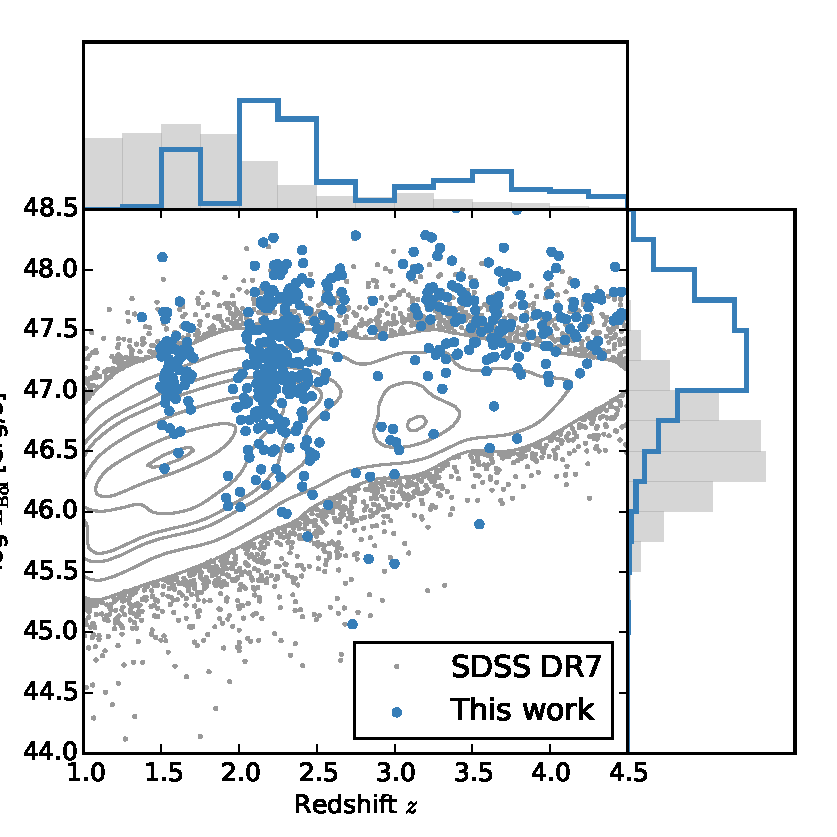
\includegraphics[width=0.8\textwidth]{figures/chapter02/luminosity_z.pdf} 
    \caption{The ranges in redshift and luminosity covered by our sample, relative to the redshift-luminosity distribution of the SDSS DR7 quasar catalogue. In regions of high point-density, contours show equally-spaced lines of constant probability density generated using a Gaussian kernel-density estimator. For the SDSS sample we use \citet{hewett10} redshifts and bolometric luminosities measured by \citet{shen11}. For the quasars in out sample the redshift is defined using the peak of the \hans/\hb emission and the luminosity is measured in the continuum at 1350\AA\, and converted to a bolometric quantity using the same conversion factor employed by \citet{shen11}. \todoinline{Eight objects are missing because we do not have enough information to calculate the bolometric luminosity.}}     
    \label{fig:lzplane}
\end{figure}


\section{Data}

The near-infrared spectra in our database are taken from published catalogues, by downloading and reducing
archival spectra, and by reducing spectra acquired in programmes led by Prof. J. Hennawi (UCSB) and Prof. X. Prochaska (UCO/LICK). 
As the P.I. of two programmes, I filled in an under-sampled region of the \ion{C}{IV} blueshift parameter space by targeting quasars with the most extreme \ion{C}{IV} blueshifts.
The telescopes and instruments used to observe these spectra are summarised in Table~\ref{tab:data_summary} and the information on the individual spectra is provided in Table~\ref{tab:database}.
In the remaineder of this chapter I will describe each of these sub-samples in turn. 

\begin{table}
  \small
  \centering
  \caption{Summary of near-infrared spectroscopic database.}
  \label{tab:data_summary}
    \begin{tabular}{cc} 
    \hline
    Instrument & Number \\  
    \hline
    FIRE/Magellan   & 36 \\
    GNIRS/Gemini    & 29 \\
    ISAAC/VLT       & 13  \\
    LIRIS/WHT       & 21  \\
    NIRI/Gemini     & 31 \\
    NIRSPEC/Keck    & 3   \\ 
    SINFONI/VLT     & 84 \\
    SofI/NTT        & 111 \\
    TRIPLESPEC/ARC  & 38 \\
    TRIPLESPEC/Hale & 60 \\
    XSHOOTER/VLT    & 36  \\
    \hline
    Total & 462 \\
    \hline
    \end{tabular}
\end{table}

\subsection{Coatman et al. (2016) Quasars}

\subsubsection{Defining sample}

We selected quasars from the SDSS DR7 spectroscopic quasar catalogue. 
The sample was restricted to objects with redshifts $2.14 < z <2.51$ (7,258 quasars), to ensure that the \hb and \ha emission lines fall within the $H$- and $K$-bands respectively, allowing us to observe both simultaneously with the appropriate grism configuration.
Given the limited number of quasars for which near-infrared spectra could be obtained, the quasar sample was further restricted to objects that are radio-quiet (5,980 quasars), show no evidence of broad absorption lines (BALs) in their spectra (5,299 quasars), and are free from significant dust extinction. 
We removed radio-loud objects from our sample using the same radio-loud classification as \citet{shen11}, and BAL quasars using the classifications of both \citet{shen11} and \citet{allen11}. 
The removal of quasars with significant dust extinction was achieved by identifying quasars with $i-K$ colours redder than a parametric spectral energy distributions (SED) model + SMC-like extinction curve with \ebv=0.05 (the SED model is described in Chapter~\ref{ch:sed}). 

The $K$-magnitude was taken from the UKIRT Infrared Deep Sky Survey \citep[UKIDSS;][]{lawrence07} Large Area Survey (ULAS). 
The requirement to be in the ULAS footprint and have reliable $K$ band photometry reduced our sample of possible targets to 1,683, and the \ebv\, cut left 1,204 in our sample. 
Finally, a flux-limit of $K<18.5$ (AB) was applied to ensure that spectra of sufficient signal-to-noise ratio (S/N) could be obtained (412 quasars). 
 
We were able to obtain new infra-red spectra for 19 quasars from this sample of 412 possible targets. 
The quasars included in this sub-sample were selected to have \ion{C}{IV}-emission shapes which span the full range observed in the population.
Reliably quantifying the distribution of \ion{C}{IV}-emission shapes has been made possible thanks to improvements in the estimation of systemic redshifts from ultraviolet spectra. 
The Allen \& Hewett (2017, in preparation) redshift estimation algorithm generates redshifts which are independent of the \ion{C}{IV}-emission shape.
This has been a crucial factor in allowing us to quantify the distribution of \ion{C}{IV}-blueshifts in the observed quasar population as a whole, and thus select a sample of quasars with a range of \ion{C}{IV} blueshifts (see Section XX). 
\todo{This paragraph could be more succinct}

\subsubsection{Observations}

Near-infrared spectra were obtained with the Long-slit Intermediate Resolution Infrared Spectrograph \citep[LIRIS;][]{manchado98} mounted on the 4.2m William Herschel Telescope (WHT) at the Observatorio del Roque de los Muchachos (La Palma, Spain). 
Observations took place over four non-contiguous nights from 2015 March 31 to April 4. 
Approximately one night was lost due to poor weather and a further half-night was affected by poor transparency due to cloud. 
A one arcsecond slit-width was employed and the LIRIS $H+K$ low-resolution grism was selected, which covers the spectral ranges 1.53--1.79\,$\mu$m and 2.07--2.44\,$\mu$m with a dispersion of 9.7\AA/pixel. 
The spatial scale of the instrument is 0.25 arcsec/pixel. 
Observations were divided into 60\,s sub-exposures and performed in an ABBA nodding pattern, with the object placed at two positions along the slit 12 arcsec apart. 
Bright A0-5V stars were observed at similar air-masses to the targets in order to provide both telluric absorption corrections and a flux calibration of the quasar spectra.

\subsubsection{Data reduction}

The raw LIRIS data frames incorporate a known `pixel shift' which was first removed from all frames using the LIRIS data reduction package {\tt LIRISDR}. 
Subsequent data reduction was undertaken with standard {\tt IRAF}\footnote{IRAF is distributed by the National Optical Astronomy Observatory, which is operated by the Association of Universities for Research in Astronomy (AURA) under a cooperative agreement with the National Science Foundation.} procedures.  
The flat-field images, which were taken at the beginning of each night via illumination of the dome, were averaged and normalised to remove any wavelength-dependent signature. 
Each individual two-dimensional spectrum was then flat-field corrected. 
Consecutive AB and BA pairs of two-dimensional spectra were subtracted to remove the sky background. 
All the subtracted AB/BA-pairs for a target were then averaged to give the final two-dimensional spectrum.

The size of the one-dimensional spectrum extraction windows, in the slit direction, varied from 6-10 pixels. 
To increase the S/N, optimal variance-weighted extraction with sigma clipping was employed. 
For the fainter objects in our sample we were unable to trace the spectrum across the dispersion axis reliably and the trace from a telluric standard-star observation, observed at a similar air mass and time, was used instead. 
The wavelength calibration, using argon and xenon lamp exposures, resulted in root mean square errors in the range 1.01--1.71\,\AA, with a mean of 1.47\AA. 
The telluric standard star observations were reduced using the same steps described above. 
The stellar continuum was divided out of the standard star spectrum, which was then divided into the quasar spectrum to remove telluric absorption features. 
The spectral type and magnitude of the standard star were used to flux calibrate the quasar spectrum both in a relative and absolute sense.
Variable atmospheric conditions combined with the narrow slit width resulted in a significant level of uncertainty in the absolute flux calibration for the quasar observations. 
The use of the UKIDSS broadband magnitudes ($H$ and $K$) to normalise the spectra results in a significantly improved calibration. 
\footnote{The data reduction pipeline is available at github.com/liamcoatman/SpectraTools}

\subsection{Shen \& Liu (2012) and Shen (2016) Quasars}

\citet{shen16a} and \citet{shen12} obtained near-infrared spectroscopy for a sample of 74 luminous, $1.5 < z < 3.5$ quasars selected from the SDSS DR7 quasar catalogue. 
Targets had to possess good optical spectra covering the \ion{C}{IV} line and have redshifts $z\sim$ 1.5, 2.1, and 3.3 to ensure that the \hbns-[\ion{O}{iii}] region was covered in one of the near-infrared $JHK$ bands.
Thirty-eight of the quasars were observed with TripleSpec \citep{wilson04} on the Astrophysics Research Consortium (ARC) 3.5\,m telescope, and 36 with the Folded-port InfraRed Echellette \citep[FIRE;][]{simcoe10} on the 6.5\,m Magellan-Baade telescope.
The reduction of the spectra is described in \citet{shen16a} and \citet{shen12}. 

\subsection{Quasar Pairs}

A large part of our catalogue was observed as part of an ongoing effort to identify quasar pairs at very close projected separations \citep[Quasars Probing Quasars\footnote{www.ucolick.org/\textasciitilde xavier/QPQ/Quasars\_Probing\_Quasars} (QPQ);][]{hennawi06a,hennawi10}. 
The primary science driver of this work is to study the circum-galactic medium of the foreground quasars in absorption \citep{hennawi06b}.
Very accurate systemic redshift measurements are a requirement and a large amount of effort has gone into obtaining near-infrared spectra which cover low-ionisation broad lines or features from the quasar narrow line region \citep{prochaska09,lau15,hennawi15}. 
Twenty-nine quasars were observed with the Gemini Near-Infrared Spectrograph \citep[GNIRS;][]{elias06} on the 8.1 m Gemini North telescope, thirtenn using the Infrared Spectrometer And Array Camera \citep[ISAAC;][]{moorwood98b} on the European Southern Observatory (ESO) Very Large Telescope (VLT), thirty-one with the Near InfraRed Imager and Spectrometer \citep[NIRI;][]{hodapp03} also on Gemini North and thirty-six with XSHOOTER \citep{vernet11}, again, on the VLT. 

The  XSHOOTER  spectra  were  reduced  with  a  custom  software  package  developed  by  George  Becker \citep[for details, see][]{lau15}. 
The remaining data was processed with algorithms in the LowRedux\footnote{www.ucolick.org/\textasciitilde xavier/LowRedux} package \citep[see][]{prochaska09}.

\subsection{VLT SINFONI Quasars}

We performed a search of the ESO archive for high-redshift quasars observed with the SINFONI  integral  field  spectrograph \citep{eisenhauer03,bonnet04} at VLT/UT4.
We found 79 quasars with redshifts $1.5 < z < 3.7$ which have $H$ and/or $K$ SINFONI spectroscopy, covering the \hb and \ha lines respectively. 
Seventy-two of the quasars are from a large programme led by L. Wisotzki (programme 083.B-0456(A)) to study the mass function and Eddington ratios of active BHs at redshifts $z\sim 2$ drawn from the Hamburg/ESO survey \citep{wisotzki00}.
A further seven SINFONI spectra are from a programme led by  J. D. Kurk (programme 090.B-0674(B)) to obtain reliable BH mass estimates from \hans/\hb for a sample of radio-loud/radio-quiet SDSS quasars.

The SINFONI spectra were reduced using the package EASYSINF\footnote{www.mrao.cam.ac.uk/\textasciitilde rw480/easysinf}.  
The package, which is based on the ESO-SINFONI pipeline, is described in \citet{williams16}. 

\subsection{ESO NTT SOFI Quasars}

One quarter of the quasar catalogue derives from a large programme (programme 187.A-0645; PI: J. Hennawi) to combine near-infrared spectra from SOFI \citep{moorwood98a} on the 3.6\,m New Technology Telescope (NTT) with archival high-resolution optical spectra from the UV-Visual Echelle Spectrograph \citep[UVES;][]{dekker00} at VLT/UT2 and the High Resolution Echelle Spectrometer \citep[HIRES;][]{vogt94} at Keck to construct a legacy database of bright, high-redshift ($2 < z < 4$) quasars with both rest-frame optical spectra, covering the \hbns-[\ion{O}{III}] complex, and high-resolution rest-frame ultraviolet spectra.
The main science goal is to obtain precise systemic redshifts which are crucial for the study of absorption line systems.  
Observations were undertaken over 16 nights from September 2011 to March 2013.
I reduced these spectra using a custom pipeline using algorithms in the LowRedux package and, in \citet{coatman17}, published a subset of the data for the first time. 

Over five nights from 2015 August 31 to September 4 we obtained near-infrared SOFI spectra for a further 26 quasars (programme 095.B-0644(A); PI: L. Coatman). 
\todo{Expand section?}
These quasars were selected from the SDSS DR7 quasar catalogue using criteria very similar to those described above for the WHT sample. 
In particular, we selected quasars with large \ion{C}{IV} blueshifts to improve the statistics in this region of the \ion{C}{IV} emission-line parameter space. 
The spectra were reduced using the same LowRedux pipeline. 

\subsection{Hale TripleSpec Quasars}

A further sixty quasars in our catalogue are bright SDSS quasars which were observed with the TRIPLESPEC spectrograph on the Palomar 200-inch Hale telescope (P200). 
The objects were observed with the same science goals as the SOFI NTT large programme. 
The spectra were reduced using a custom pipeline, again using algorithms in the LowRedux package. 

\begin{landscape}% Landscape page
    \centering % Center table
    \begin{minipage}{\linewidth}
    \small
    \renewcommand\footnoterule{}
    \captionof{table}{Quasars in our near-infrared spectroscopic database. Only the first 15 entries are shown. The full table (including 462 objects) is available online. Columns are as follows: (1) identifier, (2) date near-infrared spectra acquired, (3)-(4) coordinates, (5) instrument/telescope, (6) wavelength coverage, (7) velocity per pixel, (8) S/N per pixel, (9)-(11) redshifts from peak of [\ion{O}{III}], \hans, and \hb - see Chapter~\ref{ch:nlr} for details.}
    \label{tab:database}
    \begin{tabular}{ccccccccccc} 
    \toprule
     ID &        Date &             Ra &            Dec &            Instr. &  $\Delta\lambda$ [$\mu$m] &  $\Delta v$ [\kms] & S/N &  $z$([\ion{O}{III}]) & $z$(\hans) & $z$(\hbns) \\
     (1) &        (2) &             (3) &            (4) &            (5) &  (6) &  (7) & (8) &  (9) & (10) & (11) \\
    \midrule
     J000039-001804 &  2015-09-02 &  +00h00m39.00s &  -00d18m03.90s &         SofI/NTT &  1.50-2.54 &     154.0 &   4.9 &         &  2.1412 &  2.1391 \\
 J000345-232353 &  2009-07-07 &  +00h03m45.00s &  -23d23m53.40s &      SINFONI/VLT &  1.44-1.87 &      36.0 &  12.7 &  2.2657 &         &  2.2653 \\
 J000345-232353 &  2011-09-18 &  +00h03m45.00s &  -23d23m53.40s &         SofI/NTT &  1.48-1.83 &      63.0 &  36.0 &  2.2644 &         &  2.2776 \\
 J000451-084450 &  2013-07-12 &  +00h04m50.66s &  -08d44m49.63s &     XSHOOTER/VLT &  0.31-2.28 &      15.0 &  10.3 &  3.0038 &         &  3.0052 \\
 J000451-084452 &  2013-08-08 &  +00h04m50.91s &  -08d44m51.98s &     XSHOOTER/VLT &  0.31-2.28 &      15.0 &   5.4 &  2.9991 &         &         \\
 J000500-003348 &  2015-09-01 &  +00h05m00.42s &  -00d33m48.20s &         SofI/NTT &  1.50-2.54 &     154.0 &   8.2 &         &  2.1842 &  2.1850 \\
 J000501+010221 &  2015-09-02 &  +00h05m00.53s &  +01d02m20.80s &         SofI/NTT &  1.50-2.54 &     154.0 &   6.8 &         &  2.1334 &  2.1317 \\
 J001016+001228 &  2015-09-04 &  +00h10m16.49s &  +00d12m27.60s &         SofI/NTT &  1.50-2.54 &     154.0 &   8.9 &         &  2.2855 &  2.2828 \\
 J001247+001239 &  2013-06-06 &  +00h12m47.12s &  +00d12m39.49s &        ISAAC/VLT &  1.52-1.60 &      15.0 &  19.1 &         &         &  2.1618 \\
 J001708+813508 &  2012-08-04 &  +00h17m08.48s &  +81d35m08.10s &  TRIPLESPEC/Hale &  0.94-2.80 &      39.0 &  36.5 &  3.3934 &         &         \\
 J001919+010152 &  2015-09-04 &  +00h19m19.31s &  +01d01m52.20s &         SofI/NTT &  1.50-2.54 &     154.0 &   6.5 &  2.3120 &  2.3158 &  2.3154 \\
 J001955-091316 &  2004-11-26 &  +00h19m54.67s &  -09d13m16.45s &     GNIRS/Gemini &  0.60-2.61 &      88.0 &   9.9 &         &  2.1207 &  2.1308 \\
 J002018-233654 &  2009-07-07 &  +00h20m18.41s &  -23d36m53.80s &      SINFONI/VLT &  1.44-1.87 &      36.0 &  16.9 &  2.2975 &         &  2.2931 \\
 J002023-414639 &  2009-07-08 &  +00h20m23.38s &  -41d46m38.90s &      SINFONI/VLT &  1.09-1.41 &      35.0 &  33.4 &  1.5733 &         &  1.5730 \\
 J002111-242247 &  2009-07-16 &  +00h21m10.90s &  -24d22m47.20s &      SINFONI/VLT &  1.44-1.86 &      36.0 &  11.1 &  2.2622 &         &  2.2595 \\
    \bottomrule
    \end{tabular}
    \end{minipage}
\end{landscape}
